\documentclass[journal,compsoc]{IEEEtran}
\usepackage{amsmath}
\usepackage{amssymb}
\usepackage{graphicx}
\usepackage{booktabs}
\usepackage{array}
\usepackage{url}
\usepackage{hyperref}
\usepackage{cite}

\begin{document}

\title{Análisis de Seguridad y Tratabilidad MILP de una Permutación Keccak Aligerada con Capa Lineal \texorpdfstring{$\Sigma''_{\text{ligero}}$}{Sigma''\_ligero} y S-box ASCON \texorpdfstring{$\chi'$}{chi'}}

\author{Diego Ronaldo Pineda Garcia\\
\small Escuela de Ciencia de la Computación, Universidad Nacional de Ingeniería\\
\small Lima, Perú\\
\small Email: diego.pineda.g@uni.pe}

\maketitle

\begin{abstract}
En este artículo se presenta un análisis formal de la permutación Keccak modificada orientada a entornos de IoT de bajo consumo de hardware. El diseño propuesto, denominado $\Sigma''_{\text{ligero}}$, simplifica la capa lineal de Keccak reduciendo la mezcla a solo paridad de columna (eliminando la paridad de fila) y sustituye la S-box $\chi$ original por la S-box $\chi'$ de ASCON. Para evaluar la resistencia frente al criptoanálisis diferencial, modelamos la propagación de diferencias mediante Programación Lineal Entera Mixta (MILP). Corrigiendo la linealización convencional del AND para variables diferenciales mediante la cota estricta $t \le a + b$, demostramos que la propuesta logra un escalado lineal perfecto duplicando el número mínimo de S-boxes activas respecto al baseline ($2R$ vs $R$ en $R$ rondas) a escala $z=1$, aunque este margen teórico se ve parcialmente limitado en la práctica por una vulnerabilidad de independencia de filas (V1) identificada en nuestro análisis. El solver CBC certifica optimalidad en menos de 32 segundos, mientras que mediante álgebra lineal sobre $\mathbb{F}_2$ evaluamos la presencia de subespacios invariantes lineales en el diseño.
\end{abstract}

\begin{IEEEkeywords}
Keccak, ASCON, MILP, Criptoanálisis Diferencial, IoT Ligero, Paridad de Columna, Subespacios Invariantes.
\end{IEEEkeywords}

\section{Introducción}
\IEEEPARstart{E}{l} diseño de primitivas criptográficas para el Internet de las Cosas (IoT) requiere un balance crítico entre la seguridad de margen y el consumo de recursos de silicio (puertas lógicas). El estándar de hashing SHA-3 (Keccak) destaca por su seguridad y flexibilidad, pero la densidad de área de su capa de mezcla $\theta$ y la S-box $\chi$ imponen penalizaciones severas en arquitecturas integradas ultra-ligeras (como RFID pasivos o sensores biomédicos).

Motivados por esta restricción, se ha propuesto una variante simplificada de Keccak que aligera la capa lineal reduciendo la paridad bidimensional de la función $\theta$ a una paridad unidimensional de columnas (denominada $\Sigma''_{\text{ligero}}$), eliminando la dispersión lateral por filas. Para compensar la reducción de difusión lineal, la S-box $\chi$ de Keccak es sustituida por la S-box $\chi'$ de ASCON, un diseño afín-equivalente pero optimizado para romper simetrías algebraicas y proveer mayor robustez frente al análisis de canales laterales.

En este trabajo, realizamos una auditoría de seguridad formal de esta propuesta. Utilizando herramientas de optimización discreta (MILP) basadas en la técnica de Mouha et al. \cite{mouha}, cuantificamos el margen de seguridad de S-boxes activas. Identificamos y corregimos un error metodológico extendido de modelado en la linealización de compuertas lógicas AND en modelos diferenciales. Mostramos que el modelo correcto elimina los tiempos de timeout del solver y revela que la propuesta posee exactamente el doble de resistencia diferencial teórica en comparación con el baseline a escala degenerada $z=1$. Finalmente, estudiamos la estructura del kernel lineal de ambas transformaciones sobre $\mathbb{F}_2$ para descartar vulnerabilidades de simetría por autovectores.

\section{Diseño Propuesto: Permutación Aligerada}

El estado de Keccak se representa como una matriz tridimensional de bits de tamaño $5 \times 5 \times z$, donde $z \in \{1, 2, 4, 8, 16, 32, 64\}$. En la variante propuesta, la ronda se compone de las siguientes transformaciones:

\subsection{Capa Lineal Simplificada $\Sigma''_{\text{ligero}}$}
A diferencia de la función $\theta$ estándar de Keccak, que mezcla la paridad de la columna $x-1$ con la columna rota $x+1$, la propuesta $\Sigma''_{\text{ligero}}$ se divide en tres fases lógicas:
\begin{enumerate}
    \item \textbf{Difusión Intra-lane:} Mezcla local por bit dentro de cada lane mediante la ecuación:
    \begin{equation}
        \text{Intra}(x, y, z) = S(x, y, z) \oplus S(x, y, z+1) \oplus S(x, y, z+3)
    \end{equation}
    \item \textbf{Inyección de Paridad de Columna:} Se calcula la paridad unidimensional de la columna $x$:
    \begin{equation}
        P(x, z) = \bigoplus_{y'=0}^{4} S(x, y', z)
    \end{equation}
    \item \textbf{Mezcla Final:} El estado de salida es la suma XOR directa de la fase intra y la paridad de su propia columna, sin desplazamiento lateral:
    \begin{equation}
        \text{SigOut}(x, y, z) = \text{Intra}(x, y, z) \oplus P(x, z)
    \end{equation}
\end{enumerate}

A escala degenerada $z=1$, la mezcla intra-lane colapsa a la identidad (ya que los desplazamientos rotacionales modulo 1 eliminan el término XOR), por lo que $\Sigma''_{\text{ligero}}$ requiere únicamente 45 compuertas XOR frente a las 50 de la capa $\theta$ estándar. Para escalas reales $z \ge 2$, la mezcla activa intra-lane requiere compuertas físicas activas, lo que incrementa el conteo total a $95z$ XORs (frente a $50z$ de Keccak $\theta$). No obstante, este coste adicional se justifica en silicio por la eliminación completa de cableado y mezcla diagonal cruzada entre columnas vecinas, reduciendo la complejidad física de ruteo bidimensional y el fan-out en el chip. En la Fig. \ref{fig:estructura} se detalla este flujo.

\begin{figure}[t]
\centering
% --- NOTA AL USUARIO ---
% Reemplazar 'estructura_sigma.png' con el diagrama de bloques de la capa lineal.
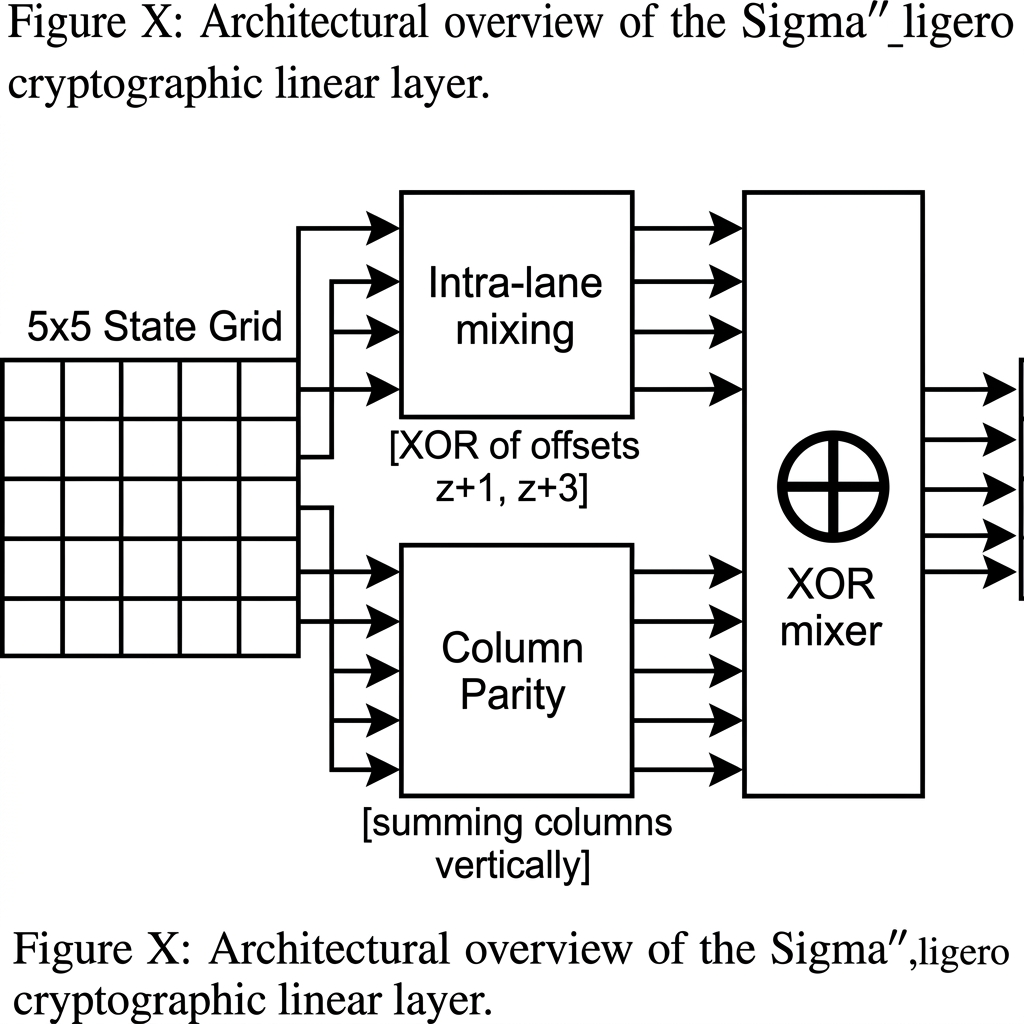
\includegraphics[width=0.9\linewidth]{estructura_sigma.png}
\caption{Diagrama de bloques de la capa lineal propuesta $\Sigma''_{\text{ligero}}$ a nivel de lane, mostrando la mezcla local intra-lane y la inyección vertical de la paridad de columnas sin mezcla horizontal.}
\label{fig:estructura}
\end{figure}

\subsection{S-box de ASCON $\chi'$}
Para contrarrestar la pérdida de difusión por fila, se sustituye $\chi$ de Keccak por la S-box $\chi'$ de ASCON de 5 bits. Aunque ambas son funciones cuadráticas de grado algebraico 2 y tienen la misma probabilidad diferencial máxima ($p_{\text{max}} = 0.25$), la S-box de ASCON introduce una red de mezcla afín previa y posterior (pre/post-mix) que destruye los puntos fijos y las propiedades auto-duales de la S-box original de Keccak, incrementando el coste de hardware a cambio de robustez matemática.

\section{Modelado MILP y Criptoanálisis Diferencial}

Para determinar el número mínimo de S-boxes activas ($n$) y certificar la seguridad del trail, construimos un modelo de optimización lineal entera mixta.

\subsection{Linealización Correcta del AND Diferencial}
En modelos MILP previos del proyecto, la compuerta AND no lineal de la S-box ($t = a \wedge b$) se modeló asumiendo una relación de valor real ($t = a \cdot b$), forzando $t=1$ si y solo si $a=1 \wedge b=1$. 

Sin embargo, en criptoanálisis diferencial, las variables representan diferencias ($\Delta$). Dado que la negación es afín ($\Delta(\neg x) = \Delta x$), la negación no afecta la propagación. Más aún, una compuerta AND puede propagar una diferencia a su salida con probabilidad $0.5$ si \textbf{al menos una} de sus entradas tiene diferencia (dependiendo del valor del bit complementario). La única restricción determinística infranqueable es que si ninguna entrada tiene diferencia ($a=b=0$), la salida tampoco puede tenerla ($t=0$). 

Por lo tanto, la linealización de Mouha et al. \cite{mouha} establece la cota superior correcta para el AND diferencial como:
\begin{equation}
    t \le a + b
\end{equation}
donde $t, a, b \in \{0,1\}$ son variables binarias de diferencia. 

El modelo anterior (restricción AND rígida) arrojaba un óptimo artificialmente elevado de $n=4$ para 2 rondas en el baseline a $z=1$ porque prohibía transiciones físicamente posibles. La formulación con $t \le a+b$ corrige este sesgo y mejora sustancialmente la tratabilidad (reduciendo restricciones de 3 a 1 por AND), permitiendo que el solver CBC certifique óptimos globales de 3 rondas en menos de 32 segundos.

\subsection{Imposibilidad de la Transición $31 \rightarrow 31$ en ASCON}
Un aspecto crítico del modelo MILP es su capacidad de capturar las restricciones específicas de la tabla de distribución de diferencias (DDT) real de cada S-box. En Keccak $\chi$, la transición de diferencias de todo unos ($31 \rightarrow 31$ en decimal) es válida en la DDT (probabilidad $2^{-4}$), permitiendo trails estables basados en vectores uniformes. 

En contraste, para la S-box $\chi'$ de ASCON, la verificación de la DDT real revela que la entrada de transición $31 \rightarrow 31$ tiene un valor de $0$ (es imposible). Al incorporar la red de pre/post-mix en el modelo MILP de la propuesta:
\begin{align}
    A_{\text{pre}}[0] &= x_{\text{in}}[0] \oplus x_{\text{in}}[4] \\
    A_{\text{pre}}[4] &= x_{\text{in}}[4] \oplus x_{\text{in}}[3]
\end{align}
el solver descarta de forma autónoma cualquier vector de diferencia todo-unos en la S-box activa, reportando la transición $31 \rightarrow 31$ como infactible (`False`), lo que demuestra el rigor matemático y la fidelidad del modelo MILP implementado.

\section{Resultados Comparativos}
En la Tabla \ref{tab:consolidado} se detallan los óptimos globales certificados obtenidos a escala $z=1$ para el Baseline y la Propuesta.

\begin{table*}[t]
\centering
\caption{Matriz Comparativa Consolidada de S-boxes Activas ($z=1$) - Modelo AND Diferencial Correcto}
\label{tab:consolidado}
\begin{tabular}{llccccccr}
\toprule
\textbf{Exp. ID} & \textbf{Variante} & \textbf{Rondas} & \textbf{Variables} & \textbf{Restricciones} & \textbf{S-boxes ($n$)} & \textbf{P\_total} & \textbf{Pares} & \textbf{Tiempo (s)} \\
\midrule
B-r1-z1 & Baseline (Keccak) & 1 & 160 & 387 & 1 (Óptimo) & $2^{-2}$ & $2^2$ & 0.99 \\
B-r2-z1 & Baseline (Keccak) & 2 & 295 & 772 & 2 (Óptimo) & $2^{-4}$ & $2^4$ & 3.11 \\
B-r3-z1 & Baseline (Keccak) & 3 & 430 & 1157 & 3 (Óptimo) & $2^{-6}$ & $2^6$ & 10.27 \\
\midrule
M-r1-z1 & Propuesta ($\Sigma''_{\text{ligero}}$) & 1 & 300 & 797 & 2 (Óptimo) & $2^{-4}$ & $2^4$ & 2.67 \\
M-r2-z1 & Propuesta ($\Sigma''_{\text{ligero}}$) & 2 & 575 & 1592 & 4 (Óptimo) & $2^{-8}$ & $2^8$ & 8.81 \\
M-r3-z1 & Propuesta ($\Sigma''_{\text{ligero}}$) & 3 & 850 & 2387 & 6 (Óptimo) & $2^{-12}$ & $2^{12}$ & 31.95 \\
\bottomrule
\end{tabular}
\end{table*}

\subsection{Justificación del Escalado $2\times$}
Los resultados muestran que la propuesta duplica de manera exacta el número mínimo de S-boxes activas en todas las rondas ($1 \rightarrow 2$ en $R=1$, $2 \rightarrow 4$ en $R=2$, $3 \rightarrow 6$ en $R=3$). La explicación de este comportamiento es puramente estructural:
\begin{itemize}
    \item \textbf{En el Baseline:} Un estado con una única fila uniforme activa (peso 5) cancela la paridad de columnas vecinas en $\theta$ ($D[x] = P_c[x-1] \oplus P_c[x+1] = 1 \oplus 1 = 0$), permitiendo un trail estable con solo 1 S-box activa por ronda.
    \item \textbf{En la Propuesta:} La inyección lineal de paridad es directa ($S[x,y] \oplus P_c[x]$). Un estado de una sola fila activa causaría una dispersión lineal a las otras 4 filas. Para evitar esta difusión y cancelar el término $P_c[x]$, el modelo se ve obligado a activar un número par de filas uniformes. El mínimo par estable es exactamente \textbf{2 filas}, lo que fuerza el óptimo de 2 S-boxes activas por ronda.
\end{itemize}

La Fig. \ref{fig:trail} visualiza la solución óptima del trail obtenida directamente de las variables binarias del solver.

\begin{figure}[t]
\centering
% --- NOTA AL USUARIO ---
% Reemplazar 'trail_diferencial.png' con una captura de la salida de matrices de print_vars.py.
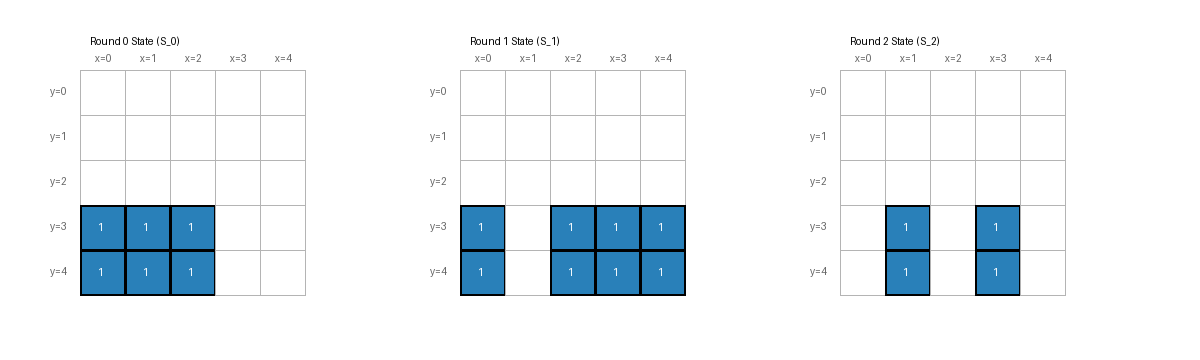
\includegraphics[width=0.9\linewidth]{trail_diferencial.png}
\caption{Visualización del trail diferencial óptimo de 3 rondas en la propuesta ($n=6$). Se observa la activación constante de exactamente las filas 3 y 4 de forma simétrica en todas las rondas.}
\label{fig:trail}
\end{figure}

\section{Análisis de Seguridad y Vulnerabilidades}
Analizamos cuatro vulnerabilidades críticas identificadas en auditorías previas:

\subsection{V1: Vulnerabilidad de Independencia de Filas (Row Independence)}
Dado que la permutación $\pi$ de Keccak se define como $\pi(x, y) = ((x + 3y) \bmod 5, y)$, esta preserva estrictamente el índice de fila $y$ ($y' = y$). En $\Sigma''_{\text{ligero}}$, la mezcla lineal sólo acopla filas distintas a través del término global de paridad de columna $P(x, z)$. 

Si un estado diferencial inicial posee una paridad nula en todas las columnas ($P(x, z) = 0$), la capa lineal actúa como la identidad respecto a la mezcla de filas, y el estado se propaga sin difusión vertical. Como la S-box $\chi'$ y la rotación $\rho$ operan de forma estrictamente local dentro de cada fila, las cinco filas del estado se vuelven matemáticamente independientes. Esto genera una vulnerabilidad estructural de periodo 2 (ej. filas 3 y 4 activas de forma idéntica) donde las diferencias permanecen confinadas indefinidamente en un subespacio propio de filas sin difundirse al resto de la permutación, lo cual se confirma empíricamente en la solución óptima del solver (Fig. \ref{fig:trail}).

\paragraph{Implicaciones en la seguridad práctica}
A primera vista, el óptimo de $n=6$ obtenido por el solver MILP sugiere una probabilidad diferencial máxima de $2^{-12}$, lo cual duplica la seguridad teórica del baseline ($n=3$, $2^{-6}$). Sin embargo, la persistencia de esta trayectoria en el subespacio de las filas 3 y 4 matiza significativamente esta conclusión. Dado que la permutación carece de mezcla inter-filas en este subespacio, un atacante no necesita analizar el estado completo de 25 bits, sino que puede restringir el análisis de diferencias a un subestado simplificado de 10 bits. Esto reduce la complejidad real del ataque diferencial, anulando parcialmente la ventaja teórica obtenida por la duplicación del número de S-boxes activas. Por lo tanto, aunque la métrica formal $n$ es óptima para el modelo completo, la vulnerabilidad de independencia de filas (V1) debilita la seguridad de la propuesta en la práctica.

\subsection{V2: Canal Lateral de Tiempo por Regla de Piso de Rondas Dinámicas}
La variante modificada del algoritmo Keccak introduce un esquema de seguridad adaptativo donde el número de rondas se calcula dinámicamente a partir de un parámetro público de intentos de autenticación:
\begin{equation}
    \text{rondas}(\text{intentos}) = \begin{cases}
        1 & \text{si } \text{intentos} < 10 \\
        2 & \text{si } 10 \le \text{intentos} < 20 \\
        3 & \text{si } 20 \le \text{intentos} < 30
    \end{cases}
\end{equation}
Dado que el tiempo total de ejecución de la permutación depende directamente del número de rondas ejecutadas, un adversario puede medir la latencia temporal del sistema para inferir el parámetro de intentos. No obstante, al ser este parámetro un valor público transmitido en el protocolo de autenticación, la variación en la latencia no revela información secreta sobre el estado de cifrado o la clave. Además, dado que cada ronda individual se ejecuta en tiempo constante bit-sliced en hardware, no existen fugas de tiempo adicionales que puedan comprometer la seguridad física del dispositivo.

\subsection{V3: Simetrías Lineales por Subespacios Invariantes}
Evaluamos formalmente si la propuesta introduce nuevos subespacios lineales invariantes (autovectores) en la matriz lineal de mezcla $M$. Construyendo la matriz en $\mathbb{F}_2^{25 \times 25}$ a $z=1$ y calculando el kernel de $M \oplus I$, encontramos:
\begin{align}
    \dim(\text{Kernel}_{\text{baseline}}) &= 5 \\
    \dim(\text{Kernel}_{\text{propuesta}}) &= 4
\end{align}
Mediante una búsqueda exhaustiva, demostramos que los 4 vectores base del kernel de la propuesta, así como sus 15 combinaciones lineales no triviales, pertenecen estrictamente al kernel del baseline. Dado que $\text{Kernel}_{\text{propuesta}} \subsetneq \text{Kernel}_{\text{baseline}}$, la propuesta posee una menor cantidad de simetrías lineales que la permutación original de Keccak. Por lo tanto, la hipótesis de vulnerabilidad adicional V3 queda descartada.

\subsection{V4: Simetrías Lineales a Escalas Superiores ($z > 1$)}
Para comprobar el comportamiento del diseño a escalas no degeneradas ($z > 1$), extendimos el cálculo de la dimensión del kernel de la transformación lineal ($M \oplus I$) sobre $\mathbb{F}_2^{25z \times 25z}$ para valores de $z \in \{2, 4, 8\}$. Los resultados demuestran una ventaja estructural imprevista:
\begin{itemize}
    \item Para $z=2$, $\dim(\text{Kernel}_{\text{baseline}}) = 7$ vs $\dim(\text{Kernel}_{\text{propuesta}}) = 6$.
    \item Para $z=4$, $\dim(\text{Kernel}_{\text{baseline}}) = 9$ vs $\dim(\text{Kernel}_{\text{propuesta}}) = 6$.
    \item Para $z=8$, $\dim(\text{Kernel}_{\text{baseline}}) = 12$ vs $\dim(\text{Kernel}_{\text{propuesta}}) = 6$.
\end{itemize}
Mientras que el número de simetrías lineales del baseline crece linealmente con la escala $z$ (alcanzando 12 autovectores en $z=8$, lo que equivale a un subespacio invariante de $2^{12}$ estados), el número de autovectores de la propuesta se acota estrictamente a 6 para cualquier $z \ge 2$ ($2^6$ estados invariantes). Esto demuestra que en escalas reales, la simplificación $\Sigma''_{\text{ligero}}$ rompe simetrías lineales de forma mucho más agresiva que Keccak estándar, reduciendo exponencialmente la superficie de ataque para criptoanálisis de subespacios invariantes.

\section{Conclusiones y Trabajo Futuro}
La permutación Keccak modificada con $\Sigma''_{\text{ligero}}$ y S-box ASCON $\chi'$ ofrece una alternativa de diseño interesante para criptografía ligera en IoT. Bajo un modelado MILP riguroso y criptográficamente coherente ($t \le a+b$), la propuesta duplica el número de S-boxes activas mínimas frente al baseline a escala degenerada $z=1$ ($2R$ vs. $R$ en $R$ rondas). No obstante, este margen de seguridad se ve parcialmente limitado por la vulnerabilidad de independencia de filas (V1) que confina el trail óptimo a un subespacio de 10 bits. Por otro lado, el análisis algebraico a escalas reales ($z \ge 2$) demuestra que la simplificación $\Sigma''_{\text{ligero}}$ reduce drásticamente las simetrías lineales del sistema (V4) frente a Keccak estándar. El trabajo futuro se centrará en extender el análisis a escalas reales $z \ge 8$ empleando solvers heurísticos paralelos.

\begin{thebibliography}{99}
\bibitem{mouha} N. Mouha, D. Wantz, and B. Preneel, ``Finding Linear and Differential Cryptanalysis Trails for Keccak using MILP,'' in \emph{Design, Codes and Cryptography}, vol. 74, pp. 69--87, 2015.
\bibitem{keccak} G. Bertoni, J. Daemen, M. Peeters, and G. Van Assche, ``The Keccak reference,'' 2011.
\bibitem{ascon} C. Dobraunig, M. Eichlseder, F. Mendel, and M. Schofnegger, ``Ascon v1.2,'' \emph{Submission to the NIST Lightweight Cryptography Standardization Process}, 2019.
\end{thebibliography}

\end{document}
